%
% Guide des themes:
% http://mcclinews.free.fr/latex/beamergalerie.php

\documentclass{beamer}
% uncomment following line for static slides 
%\documentclass[handout]{beamer}

\mode<presentation>
\mode<handout>{\beamertemplatesolidbackgroundcolor{black!5}}

\usetheme{Boadilla}
\usecolortheme{beaver}
\useinnertheme[shadow]{rounded}

%albatross -> fond bleu
%crane -> barre orang�
%beetle 
%dove fly seagull wolverine beaver

%fond ros� d�grad�
%\beamertemplateshadingbackground{red!10}{blue!10}

%\usepackage{pgf,pgfarrows,pgfnodes,pgfautomata,pgfheaps,pgfshade}

\usepackage[utf8]{inputenc}
\usepackage{eurosym}
\usepackage{pifont}
\usepackage{graphicx}
\usepackage{tabularx}
\usepackage{amsmath}
\usepackage{amsfonts}
\usepackage{comment}
\usepackage{fancyvrb}
\usepackage{pgf}
\usepackage{tikz}
% - REMARK: do not use blanks or newlines between the libraries
\usetikzlibrary{arrows,decorations.pathmorphing,decorations.footprints,fadings,shadows,decorations.text,patterns,positioning,shapes,matrix,fit}
\usepackage{calc}
\usepackage{fp} %floating point


% definition de couleur
\definecolor{gris}{rgb}{0.65,0.65,0.65}
\newcommand{\brown}[1]{\textcolor{brown}{#1}}

\usepackage{ifpdf}
        \ifpdf
          \DeclareGraphicsRule{.pdftex}{pdf}{*}{}
        \fi

\hypersetup{%
  pdfauthor={St�phane Genaud},
  pdftitle={Gestion de projet}
}

\title[Gestion Projet]{\textit{Gestion de Projet (EM615M42)}}

\author[S. Genaud]{St\'ephane Genaud }

%\AtBeginSection[]
%{
%\begin{frame}
%\frametitle{Plan section}
%\tableofcontents[currentsection]
%\end{frame}
%}


\begin{document}


\AtBeginSection[]{
  \begin{frame}
	\frametitle{Plan}
      \small \tableofcontents[currentsection, hideothersubsections]
  \end{frame} 
}


\frame{\titlepage}

%------- plan --------
\frame{
\frametitle{Plan}
\small \tableofcontents[hidesubsections]
}
%----------------------

%
\section{Le contexte de la gestion de projet}

\subsection{La notion de projet}

\frame{
\frametitle{Les origines}

\vspace{5mm}
\textbf{années 1950} : réflexion pour les grands projets industriels 
	(aéronautique, armement, travaux public)

\vspace{5mm}
\textbf{aujourd'hui} : projets de plus en plus importants (montants, internationalisation, ...)\\


\vspace{5mm}
\textbf{besoin de méthode} : constat d'échec et situation de crise
			(coûts, délais, non-fiabilité...) 

\vspace{5mm}
\textbf{influence organisationnelle} : certaines organisations
   se structurent en mode projet
\vfill
}
%*****************************************************************
\frame{\frametitle{Définition de la notion de Projet}

Un projet est une activité: 
\pause
\vspace{.2cm}
\begin{itemize}
\item<+-> unique et ponctuelle (non répétitive),\\
	    $\rightarrow$ 
	    \brown{date de début et fin du projet},
\vspace{.2cm}
\item<+-> soumise à des contraintes,\\
	    $\rightarrow$ 
	    \brown{de délais, coûts, qualité}.
\vspace{.2cm}
\item<+-> constituée d'actions ayant un objectif commun,\\
	    $\rightarrow$ 
	    \brown{nécessite des spécialistes aux compétences variées qu'il faut coordonner}, 
\vspace{.2cm}
\item<+-> qui produit un livrable\\
	    $\rightarrow$ 
	    \brown{résultat permettant la satisfaction d'un besoin identifié.}
\end{itemize}
}

%********************* Phases *************************************

\subsection{La genèse d'un projet}
\frame{\frametitle{Genèse d'un projet}


\begin{figure}[!htb]
\begin{tikzpicture}
[
      xscale      = 1,  % to scale horizontally everything but the text
      yscale      = 1,  % to scale vertically everything but the text
]

% Noeud "Besoin"
\node (besoin) [ 	shape             = circle,
            	top color         = white,        
            	bottom color      = blue!20!white, 
            	text              = blue,        
            	text width        = 1.4cm,        
            	align             = center,    
            	draw              = blue,     
            	rotate            = 2,       
            	thick,]
	at (-4,0) {Besoin};


%% --- etape 2
\only<2->{
% Noeud "Livrable"
\node (livrable) at (5,0)
	{
\includegraphics[height=1.7cm]{fig/livrable.png} Livrable};

% chemin 
\draw[dotted, ultra thick,->] (besoin) -- (livrable);
}


\onslide<3->{
\node (projet) [	shape             = rectangle,
            	top color         = white,
            	bottom color      = red!20!white, 	% |
            	text              = black,                % colour of the fonts
            	text width        = 3cm,        
            	align             = center,               % text alignment
            	draw              = red,                % colour of the border
            	align             = center,    
            	thick,]
		at (0,0) {Projet};
}

%% --- etape 4
\onslide<4->{
	\node (chefprojet) at (0,-2) {
\includegraphics[height=9mm] {fig/user_female.png}};
	\draw (0,-2.5) node[below]{{\small Chef de projet}};
	\draw[thick,->] (chefprojet) -- (projet);
}
\onslide<5->{
	\node (decideur) at (0,2) {
\includegraphics[height=9mm] {fig/user_executive.png}};
	\draw[thick,->] (decideur) -- (projet)
			    node[near start,above]{\small Décideur};
}
\onslide<6->{
	\node (equipe) at (2,-2) {
\includegraphics[height=9mm] {fig/user_group.png}};
	\draw (2,-2.5) node[below]{\small Equipes};
	\draw[thick,->] (equipe) -- (projet);
}
\end{tikzpicture}
\end{figure}
%  ______________________________________________________________________________________________
}


\subsection{La conduite du projet}
\frame{\frametitle{Conduite de projet}

La \emph{conduite de projet} est la façon dont cette démarche est menée.\\
\vspace{2cm}

C'est un cadre méthodologique qui préconise:
\begin{itemize}
\item<+-> les grandes phases d'un projet 
\item<+-> les étapes usuelles jalonnant un projet
\item<+-> les protocoles usuels entre les acteurs du projet
\end{itemize}
}

%********************* Phases *************************************
\frame{\frametitle{Les grandes phases}

\begin{itemize}
\item Définition
\item Réalisation
\item Mise en {\oe}uvre
\item Bilan 
\end{itemize}
}


%********************* Phases *************************************
\frame{
\begin{center}
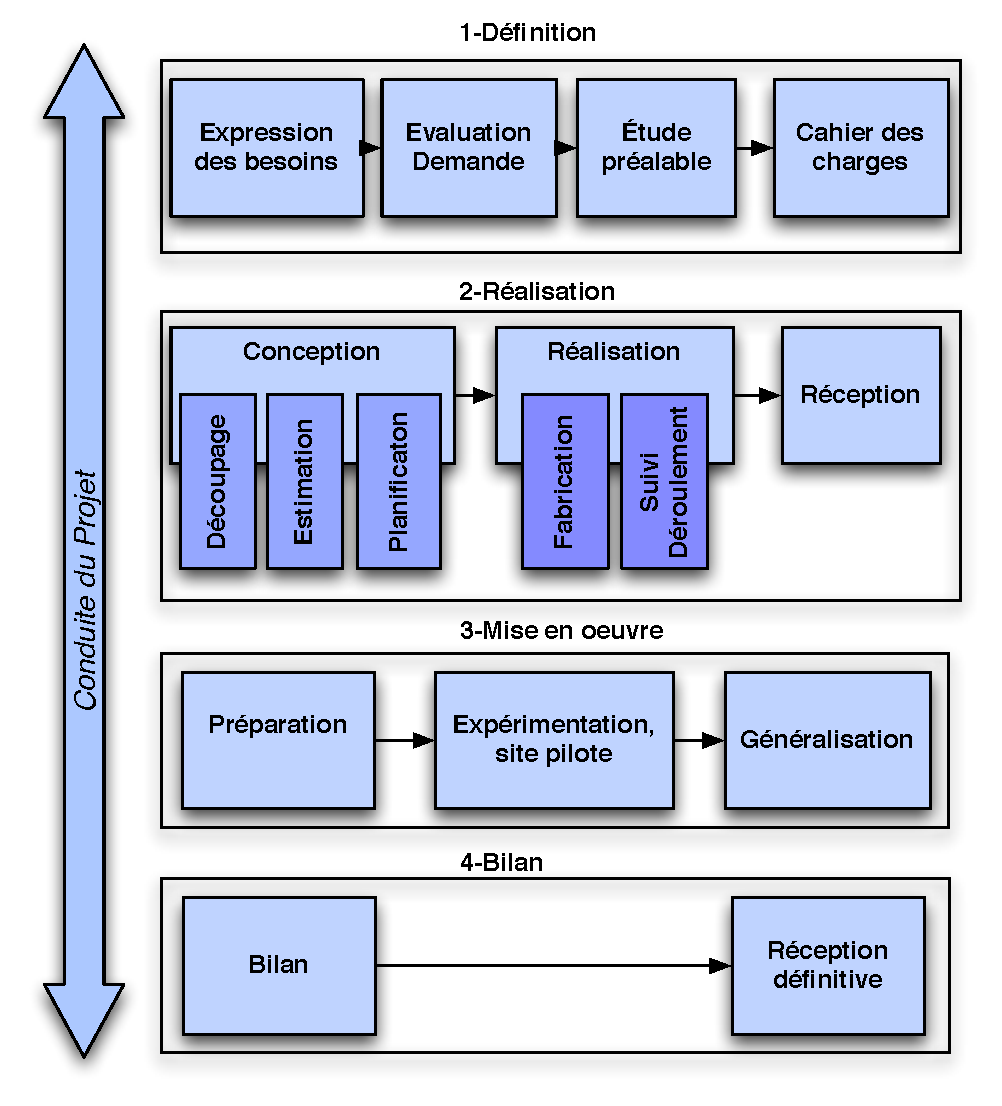
\includegraphics[height=\textheight]{overview-projet.pdf}
\end{center}
}


\subsection{Vérifier l'opportunité du projet}

%*****************************************************************
\frame{
\frametitle{Etude d'opportunité}

\onslide<1>{\center ... Avant de se lancer ...}
\pause
\begin{figure}[!htb]
\begin{tikzpicture} [xscale=1,yscale=1]

% Noeud "Besoin"
\node (besoin) [ 	shape             = circle,
            	top color         = white,        
            	bottom color      = blue!20!white, 
            	text              = blue,        
            	text width        = 1.4cm,        
            	align             = center,    
            	draw              = blue,     
            	rotate            = 2,       
            	thick,]
	at (-4,0) {Besoin};

\node (livrable) at (5,0)
	{
\includegraphics[height=1.7cm]{fig/livrable.png} Livrable};
\draw[dotted, ultra thick,->] (besoin) -- (livrable);
\node (projet) [	shape             = rectangle,
            	top color         = gray!20!white,
            	bottom color      = red!20!white, 	% |
            	text              = black,                % colour of the fonts
            	text width        = 3cm,        
            	align             = center,               % text alignment
            	draw              = red,                % colour of the border
            	align             = center,    
            	thick,]
		at (0,0) {Projet};

\node (opportunite) [shape             = rectangle,
            	top color         = white,        
            	bottom color      = red!20!white, 	% |
            	text              = black,                % colour of the fonts
            	text width        = 2cm,        
            	align             = center,               % text alignment
            	draw              = red,                % colour of the border
            	align             = center,    
            	thick,]
		at (-1.5,-1.5) {\'Etude opportunité};
\draw[ultra thick,->] (opportunite) -- (-1.8,-.1);


\end{tikzpicture}
\end{figure}
}
%  ______________________________________________________________________________________________



%*****************************************************************
\frame{
\frametitle{Etude d'opportunité}


\vspace{.5cm}
Avant acceptation ou lancement, se poser des questions :\\ 

\vspace{.5cm}
Toute difficulté identifiée devra faire l'objet 
d'un dialogue approfondi avec le demandeur pour

\begin{itemize}
\item soit annuler, infléchir ou différer le projet
\item soit négocier des moyens de réussite à hauteur des enjeux et des conditions de
réussite identifiées.
\end{itemize}

\vspace{.5cm}
$\Rightarrow$ Une \underline{évaluation} 
sous différents angles est nécessaire.
}

\frame{
\frametitle{Exemple simple: l'électricien}

\begin{block}{La demande}
Le client veut un site web pour 
\begin{itemize}
\item informer ses clients (horaires, produits, services, ...),
\item enregistrer demandes de devis, 
\item distribuer un dépliant electronique, 
\item ...
\end{itemize}
\end{block}
}

\frame{
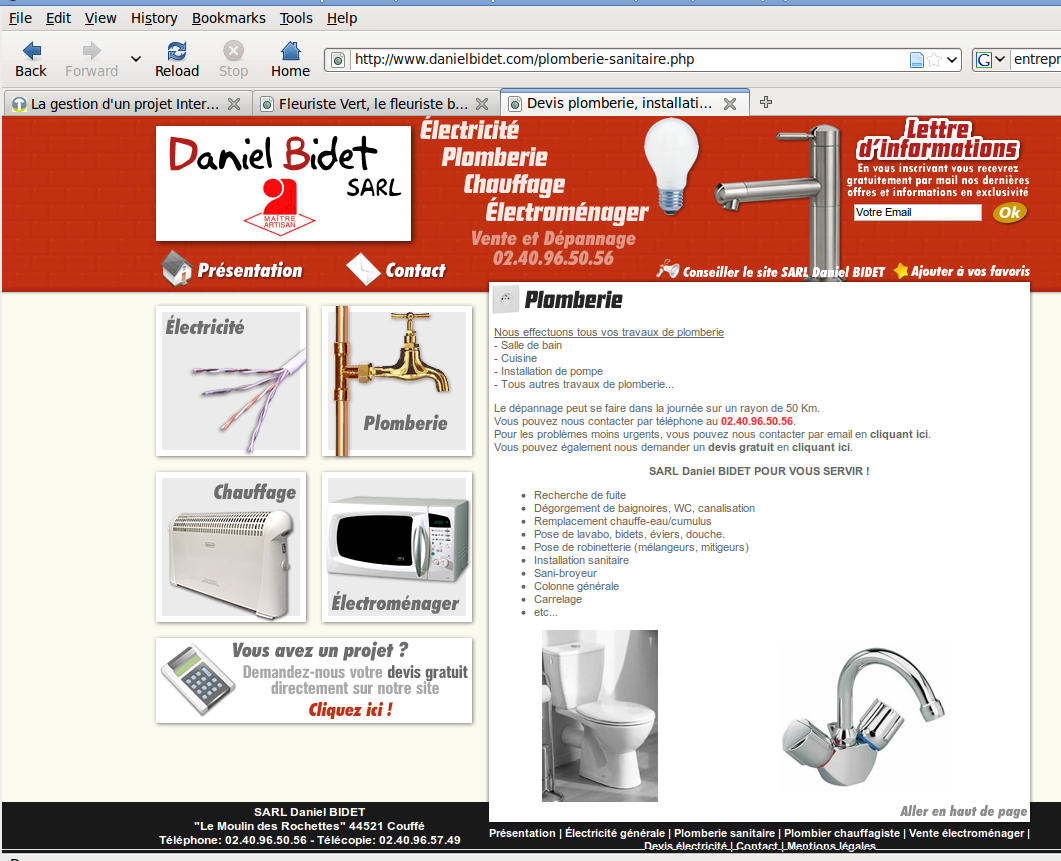
\includegraphics[width=\textwidth]{capture-site-electr.png}
}

\frame{
\frametitle{Exemple simple: l'électricien}

\begin{block}{La demande}
Le client veut un site web pour 
\begin{itemize}
\item informer ses clients (horaires, produits, services, ...),
\item enregistrer demandes de devis, 
\item distribuer un dépliant electronique, 
\item ...
\end{itemize}
\end{block}

\only<1>{Simple, non ? ...}
\only<2>{... Pourtant, répondre à cette demande nécessite de dialoguer avec le client.}

}
\frame{
\textit{
Quelques questions immédiates (liste non-exhaustive):
\begin{itemize}
    \item<+-> Qui décidera des informations nouvelles à enregistrer et publier ?
    \item<+-> Sur quels critères mettra t-on les informations produits/tarifs à jour ?
    \item<+-> De qui et comment viendront ces informations ?
    \item<+-> Qui mettra ces informations en ligne, sous quelle forme ? 
    \item<+-> Quelles compétences sont requises pour intervenir sur le site ? 
    \item<+-> Les visiteurs auront-ils le moyen d'enregistrer des alertes ? 
    \item<+-> Qui sera alerté ? Avec quels critères ? 
    \item<+-> ... Un deuxième niveau de questions devra cerner les motivations des acteurs...
\end{itemize}
}

\vspace{5mm}
\onslide<9->{Risque: un site au contenu périmé \ding{63} }
\onslide<10>{$\Rightarrow$ Adopter une démarche d'évaluation: le projet est-il clairement défini ?}
}

%*****************************************************************
\subsection{Lancement du projet: l'évaluation }
\frame{
\frametitle{Lancement du projet: l'évaluation}

Entre l'idée et sa réalisation, il peut y avoir un gouffre.
Le résultat attendu peut être flou et les implications mal cernées.  

\begin{block}{Règle 1 : Définissez l'idée en termes de résultat attendu}
    S'assurer que les décideurs sont d'accords avec ces résultats et peuvent dire ce qui va changer par rapport à ce qui est connu.

\pause
    \begin{itemize}
    \item<+-> Tous les acteurs ont ils la même représentation du produit attendu ?
    \item<+-> Cerner la demande : demande énoncée clairement, nature de la demande, cadre de la demande, les délais 
    \item<+-> Quels changements l'idée va t-elle produire ? Sont ils acceptables dans les structures et comportements ?
Que faut il faire pour les rendre acceptables ? 
    \end{itemize}
\end{block}  
}



\frame{
\frametitle{Evaluer le projet}

Le résultat attendu peut être ``contre-nature''.

\begin{block}{Règle 2 : évaluer la cohérence} 
Evaluer par la cohérence du projet dans le contexte de l'organisation
    \begin{itemize}
    \item<+-> Identifier le demandeur et protagonsites impliqués (initiateur, décideur, destinataire)
		% Ex: la demande vient des utilisateurs d'un service, relayée par le responsable du service,
		% appuyée par le chef du département et avalisée par la direction
    \item<+-> Générateur de résultats économiques ?
		% Va t-on avoir des gains ? quantifiables ?
    \item<+-> Les résultats escomptés sont ils en accord avec la stratégie de l'entreprise ? 
		% pas de contradiction avec les objectifs généraux affichés
		% Ex: l'entreprise annonce qu'elle passe d'une distrib. par revendeurs à distrib. directe mais le projet
		% concerne l'amélioration de la logistique de livraison des revendeurs
    \item<+-> Le projet s'inscrit-il dans la planification générale de l'entreprise ?
    Positionnement vis-à-vis d'autres projets ou actions ? (antinomies, synergies, compétition )
		% Ex: le projet logistique permet de livrer et d'informer les distributeurs sur les nouveaux produits mais
		% parallèlement un projet d'extranet revendeurs fournira également un catalogue et infos produits
    \end{itemize}
\end{block}
}


\frame{
\frametitle{Evaluer le projet }

Le projet peut devenir incontrôlable.

\begin{block}{Règle 3 : évaluer la conduite de projet} 
Evaluer par la conduite de projet : les risques d'aléas
    \begin{itemize}
    \item <+-> Garanties de progression et d'achèvement ? 
    \item <+-> Programme des étapes et décisions intermédiaires connus ?
    \item <+-> Les indicateurs de bonne fin sont ils précisés ?
    \end{itemize}
	
\end{block}
}

%******** CAS Personal Fit  ***************************
\frame{
\frametitle{Cas \textit{Personal Fit}}

\textbf{4.5.6} est une enseigne de prêt à porter pour femme, dont la cible est
la clientèle 30-50 ans. La marque est présente sous la forme d'un réseau de
franchisés (95 boutiques).

Elle désire lancer une offre distinctive \textit{Personal Fit}, un service de
vêtements ``sur mesure`'': une gamme spécifique de vêtements avec un choix de tailles
beaucoup plus fin, qui peut être guidé par des mesures electroniques. 

\vspace{5mm}
\begin{center}
\ldots voir étude de cas \ldots
\end{center}
}


%******************************************************************
\section{Les acteurs}
\subsection{Le triangle projet: objectifs, délais, ressources}

\frame{
\frametitle{Le triangle projet}
 
\input{triangle.pdftex_t}

\vfill                 
}

%*****************************************************************
\frame{
\frametitle{Les objectifs}

\begin{center}
	`` Quoi faire ? ''
\end{center}
Définir le domaine couvert en termes de fonctionnalités. 
Le document contractuel est le \alert{cahier des charges}.
}

\frame{
\frametitle{Les délais}
\begin{center}
	`` Quand faire ? ''
\end{center}
La gestion des délais intervient une fois les étapes de découpage et d'estimation terminées. 
Un \alert{calendrier} contractuel définissant les délivrables intermédiaires peut être établi.
}

 
\frame{
\frametitle{Les ressources}

\begin{center}
	`` Avec qui/quoi faire ? ''
\end{center}


La gestion des ressources nécessite une \alert{organisation} parfois complexe.\\

Des structurations typiques des ressources humaines sont:
\begin{itemize}
\item structuration générale \emph{client/fournisseur}.
\item structuration en \emph{maîtrise d'ouvrage/maîtrise d'{\oe}uvre}.
\end{itemize}
}

\subsection{Structurations typiques pour les ressources humaines}
%******************************************************************
\frame{
\frametitle{Structuration client/fournisseur}

Dans de nombreux projets, on peut retrouver les acteurs suivants:

\underline{parmi les clients} :
\begin{itemize}
\item les décideurs
\item le chef de projet
\item les usagers
\end{itemize}

\underline{parmi les fournisseurs} :
\begin{itemize}
\item le chef de projet
\item les concepteurs
\item les équipes de fabrication
\end{itemize}
\vfill
}
%******************************************************************

\frame{
\frametitle{Structuration maîtrise d'ouvrage/maîtrise d'{\oe}uvre}

Quand les entreprises sont structurées pour gérer des projets 
on a souvent une organisation en \textbf{maîtrise d'ouvrage} (MOA) et
 \textbf{maîtrise d'{\oe}uvre} (MOE).\\

\pause
Ce sont deux entités de l'organisation (personnes morales).
\pause

\begin{itemize}
\item<+-> Le MOA est client du MOE à qui il passe commande d'un produit nécessaire à son activité.
\item<+-> Le MOE fournit ce produit: soit il le réalise lui-même, soit il passe commande à un ou plusieurs fournisseurs qui élaborent le produit sous sa direction. 
\end {itemize} 

}

\frame{
\frametitle{Les acteurs : structuration}
\input{acteurs.pdftex_t}

}   
\frame{
\frametitle{La maîtrise d'ouvrage : 6 fonctions}
\begin{itemize}
\item<+-> le maître d'ouvrage stratégique (MOAS)\\
	$\rightarrow$ prend les décisions, arbitre.
\item<+->  le maître d'ouvrage délégué (MOAD)\\
	$\rightarrow$ fournit les éléments factuels au MOAS.
\item<+->  le maître d'ouvrage opérationnel (MOAO)\\
	$\rightarrow$ expert d'un grand processus du métier.
\item<+->  l'assistant à maîtrise d'ouvrage (AMO),\\
      $\rightarrow$ support pour le MOAO ou MOAD en période de pointe, ou quand le projet demande des compétences non maitrisées. 
\item<+->  l'expert métier,\\
      $\rightarrow$ vérifie la pertinence du produit avec les exigences des utilisateurs
\item<+->   l'utilisateur\\
       $\rightarrow$ peuvent compléter les observations de l'expert métier.
\end {itemize}

}

\frame{
\frametitle{La maîtrise d'{\oe}uvre}

Le MOE est responsable de la qualité technique de la solution. 
Il doit, avant toute livraison au MOA, 
procéder aux vérifications nécessaires (``recette usine'').\\

\vspace{1cm}
 
Pour cela, le MOE doit assurer la coordination de tous les fabriquants en veillant (entre autres):
\begin{itemize}
\item à la cohérence des fournitures et à leur compatibilité,
\item à coordonner l'action des fournisseurs en contrôlant la qualité technique,
\item à respecter les délais fixés par le MOA et en minimisant les risques.
\end{itemize}
}

  
%*****************************************************************
\begin{comment}
\subsection{Eléments de motivation}
\frame{
\frametitle{Motiver l'équipe de projet}

Chaque acteur s'engagera d'autant plus que :
 
\begin{itemize}
\item le résultat de son action est visible
\item le résultat envisagé est désiré
\item sa confiance dans sa capacité à agir est grande
\end{itemize} 


Provoquer ces trois facteurs :
\begin{itemize}
\item s'accorder sur le chemin à parcourir
\item assurer la continuité du processus
\item faire adhérer les équipes
\item agir par la hiérarchie
\item investir en ressources humaines, temps, argent
\end{itemize} 
}
\end{comment}


%\section{Le découpage}
%*****************************************************************
\subsection{Pourquoi découper ?}
\frame{
\frametitle{Pourquoi découper ?}

Le découpage est l'identification des tâches qui
vont mener à la réalisation du livrable.
\pause

\begin{itemize}
\item<+-> Faire face à la complexité des activités\\
      \brown{``diviser pour régner''}

\item<+-> Aborder le projet en termes d'unités de fabrication\\
      \brown{Toujours se souvenir de l'objectif final}
      
\item<+-> Faciliter le suivi du projet\\
      \brown{Détecter les dérives plus vite}

\item<+-> Affecter des activités aux acteurs\\
      \brown{Faire correspondre besoins et compétences}
      
\item<+-> Ordonnancer\\
      \brown{Planifier le travail sur un calendrier}
\end{itemize} 
}
%*****************************************************************
\subsection{Principe du découpage}
\frame{
\frametitle{Principes du découpage}
 
\begin{itemize}
\item<+-> \textbf{Objets} du  découpage : des éléments autonomes
 	\begin{itemize}
 	\item<+->  qui produisent un résultat final
 	\item<+->  qui ont une charge mesurable
 	\item<+->  dont on peut identifier leurs contraintes d'antériorité
	\end{itemize}
	\vspace{5mm}
\item<+-> \textbf{Approches} du découpage 
	\begin{itemize}
	\item<+-> approche temporelle : succession de phases, de jalon, $\dots$
	\item<+-> approche structurelle : définition des modules composant le livrable
	\end{itemize}
	Il faut combiner les deux approches.
\end{itemize} 
}
%*****************************************************************
\frame{
\frametitle{Difficultés du découpage}

Que se passe t-il quand on oublie d'identifier certaines tâches ?
N'oublions pas que l'objectif est contractualisé.
Quelles en sont les conséquences ?
\pause

\begin{itemize}
\item <+->Modification du calendrier et du budget.\\
 
\item <+->Demander l'aval à la maîtrise d'ouvrage.\\
\end{itemize}
}
%*****************************************************************

\subsection{S'aider d'une méthode}
\frame{
\frametitle{S'aider d'une méthode}

\begin{itemize}
\item<+->  Méthode générale, comme
\begin{itemize}
\item PBS (\emph{Product Breakdown Structure})
\item WBS (\emph{Work Breakdown Structure})
\item OBS (\emph{Organisation Breakdown Structure})
\end{itemize}
\vspace{5mm}

\item<+-> Méthode plus spécifique, caution pour une communauté :\\
      ex : Norme de conduite de projet AFNOR Z67-101
\vspace{5mm}

\item<+-> Méthodes de conception spécifique métier :\\
      Exemple pour les développements informatiques (Merise)
\end{itemize}
}

%*****************************************************************
\frame{
\frametitle{Méthodes PBS/WBS/OBS}

\begin{itemize}
\vspace{5mm}
\item 
PBS : vue hiérarchique des composants, parties, sous-parties,
nécessaires à la construction du produit.

\vspace{5mm}
\item
WBS : division hiérarchique du travail global à réaliser
en \emph{work packages} (ou \emph{lots de travail}), qui peuvent être
estimés, planifiés, et affectés à un responsable (personne ou service).

\vspace{5mm}
\item
OBS : hierarchie de l'organisation qui mène le projet, qui permet.
de mettre en relation PBS avec WBS pour identifier
les responsabilités vis-à-vis des work-packages.

\end{itemize}
}


%*****************************************************************
\frame{
\frametitle{PBS-WBS-OBS}
\begin{center}
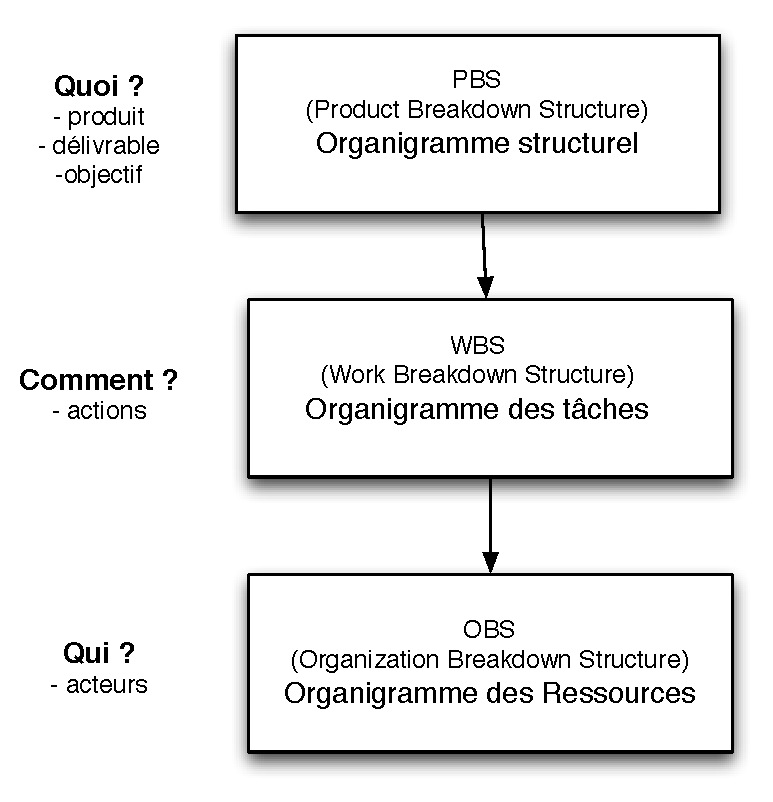
\includegraphics[height=.8\textheight]{pbs-wbs-obs.pdf} 
\end{center}
\vfill  
}
%*****************************************************************
\frame{
\frametitle{Exemple PBS (Product)}
\vspace{1cm}
Découpage PBS (formalisme graphique)
%--------------
%exportée à 70%
%--------------
\[ \input decoupe_PBS.pdftex_t \]
\vfill  
}

%*****************************************************************
\frame{
\frametitle{Exemple WBS (Work)}
\vspace{1cm}

Découpage WBS (formalisme graphique)
%--------------
%exportée à 70%
%--------------
\[ \input decoupe_WBS.pdftex_t \]

\vfill  
}
%*****************************************************************
\frame{
\frametitle{Relation OBS/WBS}
\vspace{1cm}

Relation  OBS/WBS $\Rightarrow$ Responsabilités vis-à-vis du produit

\[ \input decoupe_OWBS.pdftex_t \]

Aussi désignée par \emph{Responsibility Assignment Matrix} (RAM)
}
%*****************************************************************
\frame{
\frametitle{Exemple WBS : institut de formation}

Pour la gestion d'un institut on identifié 4 domaines:
\begin{itemize}
\item gestion des candidatures 
\item gestion des demandes de stages
\item gestion des stages
\item suivi budgétaire
\end{itemize}
Pour chaque domaine, on décrit la succession des 
travaux à mener. Par exemple:
}

\frame{
\frametitle{Exemple WBS : institut de formation}
\begin{center}
\fbox{\begin{minipage}[t]{9cm}
Application 1 : \textbf{Gestion des candidatures}\\
\begin{enumerate}
	\item[1.] Etude préalable
	\begin{enumerate}
		\item[11.] Lancement de la phase
		\item[12.] Recueil de l'existant
		\item[13.] Conception
		\item[14.] Appréciation
		\item[15.] Validation de la phase
	\end{enumerate}
	\item[2.] Etude détaillée
	\begin{enumerate}
		\item[21.] Conception fonctionnelle générale
		\item[22.] Conception fonctionnelle détaillée
		\item[23.] Conception technique validation
	\end{enumerate}
	\item[3.] Réalisation
	\begin{enumerate}
		\item[31.] Etude technique 
		\item[32.] Production du logiciel
	\end{enumerate}
\end{enumerate}
\end{minipage}
}\end{center}
 
}
%*****************************************************************
\frame{
\frametitle{exemple : institut de formation (2)}
on raffine: 
\begin{center}
\fbox{
\begin{minipage}[t]{9cm}
\begin{enumerate}
	\item[1.] Etude préalable
	\begin{enumerate}
		\item[14.] Appréciation
		\begin{enumerate}
			\item[141.] Etude des scénarios de développement
			\item[142.] Elaboration du bilan
			\item[143.] Rédaction du dossier de choix
			\item[143.] Réunion du comité directeur
		\end{enumerate}
	\end{enumerate}
\end{enumerate}
\end{minipage}
}

\vspace{.5cm}
\pause

\fbox{
\begin{minipage}[t]{9cm}
\begin{enumerate}
	\item[142.] Elaboration du bilan
	\begin{enumerate}
		\item[1421.] Recueil des éléments de coûts 
		\item[1422.] Recherche des éléments de gain attendus 
		\item[1423.] Construction des bilans par scénario 
	\end{enumerate}
\end{enumerate}
\end{minipage}
}


\end{center}
}


%*****************************************************************
\frame{
\frametitle{Synthèse WBS/PBS/OBS}

\begin{itemize}
\item La méthode est générale, et peut s'appliquer à tout projet.\\

\item Certaines spécifités du métiers
      ne sont pas prises en compte (trop générale).\\

\item La structure hiérarchique arborescente favorise un découpage
      récursif des éléments.\\
      
\item Dans la pratique, on utilise des patrons (templates) définis pour un type de projet donné.\\
Exemple : l'armée U.S. demande à ses sous-traitants de se conformer 
au WBS normalisé US MIL-STD-881.
\end{itemize}

}
%*****************************************************************
\subsection{Decoupage en phases}
\frame{
\frametitle{Découpage en phases}
On retrouve généralement les phases suivantes, terminées par une procédure de validation.

\pause

\begin{enumerate}
\item	<2,8> \textbf{\'{E}tude de faisabilité} 
\small{(ou \textbf{préliminaire}, \textbf{préalable}, \textbf{d'opportunité})}

\item	<3,8> \textbf{Lancement}

\item	<4,8> \textbf{Définition des solutions}

\item	<5,8> \textbf{Conception détaillée}

\item	<6,8> \textbf{Réalisation}

\item	<7,8>\textbf{Recette}

\end{enumerate}

%-------------------- frame etude detaillée ---------
 \only<2>{
      \begin{tabular}{|p{\textwidth}|}
      \hline
      -- dététerminer le périmètre (ce qui sera inclus dans les objectifs),\\
      -- sa faisabilité technique (e.g. étude de terrain, recherche de solution existante),\\
      -- les compétences requises, les compétences à acquérir,\\
      -- les risques de faire, les risques de ne pas faire, éventuellement le retour sur investissement attendu.\\
      \hline
      \end{tabular}
}
%-------------------- frame lancement ---------
\only<3>{
      \vspace{3mm}
      \begin{tabular}{|p{\textwidth}|}
      \hline 
      -- on définit l'organisation du projet (chef de projet, comité pilotage, experts, sous-traitants),\\
      -- les moyens de contrôler les résultats,\\
      -- les engagements budgétaires.\\
      \hline
      \end{tabular}
}

%-------------------- frame def. solution ---------
\only<4>{
      \vspace{3mm}
      \begin{tabular}{|p{\textwidth}|}
      \hline 
      -- étude de différentes solutions ou architectures techniques possibles,\\
      -- appel d'offre éventuels auprès de sous-traitants,\\
      -- réalisation d'un prototype,\\
      -- éventuellement, mise sur un marché test.\\
      \hline
      \end{tabular}
}
%-------------------- frame conception detaillee ---------
\only<5>{
      \begin{tabular}{|p{\textwidth}|}
      \hline 
      -- représentation précise de l'objectif à travers les spécifications,\\
	-- contrats de réalisation, cahier des charges fournisseurs.\\
      \hline 
      \end{tabular}
}
%-------------------- frame realisation ---------
\only<6>{
      \vspace{3mm}
      \begin{tabular}{|p{\textwidth}|}
      \hline 
	-- la fabrication même du produit final\\
      -- tests (unitaires, d'intégration, de performance)\\
      \hline 
      \end{tabular}
}
%-------------------- frame recette ---------
\only<7>{
      \vspace{3mm}
      \begin{tabular}{|p{\textwidth}|}
      \hline 
      -- vérification globale avec accompagnement (formation, conduite du changement, ...).\\
      -- réception, qualification, certification, homologation, simulation.\\
      \hline 
      \end{tabular}
}

%-------------------- fin des frames ---------
\pause
}

%*****************************************************************
\frame{
\frametitle{Norme AFNOR}

Norme Z67-101 "recommandations pour la conduite de projets informatiques"
s'inspire de la méthode Merise.

\begin{center}
\begin{small}
\begin{tabular}{|ll|}
\hline
1. \'{E}tude préalable		& $\left\{\begin{tabular}{ll}
				Exploration \\
				Conception d'ensemble\\
				Appréciation solution
			  \end{tabular}\right.$\\
\hline
2. Conception détaillée	& $\left\{\begin{tabular}{ll}
				Conception du S.I.\\
				Spécifications fonctionnelles\\
				Etude organique générale
			  \end{tabular}\right.$\\
\hline			  
3. Réalisation	& $\left\{\begin{tabular}{ll}
				Etude organique détaillée\\
				Programmation et tests\\
				Validation technique
			  \end{tabular}\right.$\\
 \hline
4. Mise en oeuvre	& $\left\{\begin{tabular}{ll}
				Réception provisoire\\
				Exploitation sous contrôle
			  \end{tabular}\right.$\\
\hline			  
5. \'{E}valuation	& $\left\{\begin{tabular}{ll}
				 Evaluation du système info.\\
				 Evaluation du S.I.
			  \end{tabular}\right.$\\\hline	  
\end{tabular}
\end{small}
\end{center}
}


%\section{L'estimation d'un projet}

%*****************************************************************
\subsection{Pourquoi estimer ?}
\frame{\frametitle{Pourquoi estimer ?}

\vspace{.5cm}
\begin{itemize}
\item Cerner la dur�e du projet\\
\vspace{.2cm}
\item D�terminer les ressources � mettre en {\oe}uvre\\
\vspace{.2cm}
\item D�terminer la faisabilit� technique du projet\\
\vspace{.2cm}
\item Pouvoir n�gocier\\
\vspace{.2cm}
\item \'{E}viter les d�rives de co�ts\\

\end{itemize}
\vfill
}
%*****************************************************************

\subsection{Estimer � diff�rents niveaux} 
\frame{\frametitle{Estimations � diff�rents niveaux}

\begin{itemize}

\item<+-> Niveau projet
 \begin{itemize}	
     \item	d�terminer enveloppe budg�taire\\
     \item	poids du projet en termes d'effort\\
     \item	estimation de la rentabilit�\\
     \item  �valuer une dur�e vraisemblable\\
 \end{itemize}

\item<+->Niveau �tape
 \begin{itemize}	
	\item ajuster le d�coupage\\
	\item sous-traiter\\
	\item pr�voir ressources\\
	\item pr�voir d�lais pour planifier l'ordonnancement\\
 \end{itemize}

\item<+-> Niveau phase
 \begin{itemize}	
	\item planification pr�cise\\
	\item calendrier des fournitures interm�diaires\\
	\item pr�voir suivi de projet \\
	\item pr�voir les mont�es/baisses en charge \\
\end{itemize}

\item<+-> Niveau t�che 
 \begin{itemize}	
	\item �valuer les t�ches (souvent individuelles)  \\
 \end{itemize}
\end{itemize}


}

%*****************************************************************
\subsection{Estimer charges et co�ts}
\frame{\frametitle{Unit� de charge}

\vspace{.5cm}
\begin{itemize}

\item
La \emph{charge} est la quantit� de travail exprim�e en $ressources \times temps$.  \\

\item Les  $ressource$ sont souvent des \textbf{hommes}\\

\item Le $temps$ est le
       \begin{itemize}
       \item[--] \textbf{mois} pour les grands projets, 
       \item[--] \textbf{jour} pour les petits projets.
       \end{itemize}

\item La charge est souvent pond�r�e par coefficient de productivit�
\end{itemize}
\vspace{.6cm}
Exemple : 10 jours $\times$ hommes \\ 
$\Leftrightarrow$ 1 homme pendant 10 jours\\ 
$\Leftrightarrow$ 10 hommes pendant 1 jour\\ 
$\Leftrightarrow$ 5 hommes pendant 2 jours\\
$\Leftrightarrow  \cdots$ \\
\vfill
}
	
%*****************************************************************
\frame{\frametitle{Unit� de charge corrig�e}
\underline{Exemple de correction de productivit�} :
\begin{center}	
	jours ouvrables $jo = 52 \times 5 = 260$
\end{center}	
	
\[\begin{tabular}{ll}
jours f�ri�s		& 12\\
cong�s			& 30 \\
maladie			& 3\\
formation		& 4\\
r�unions		& 6\\
\hline
nb jours improductifs ($ji$) =	& 55
\end{tabular}\]

 
$$ {\rm coefficient} = \frac{jo}{jo - ji}=\frac{260}{205}=1,26$$ 
 
 
\vfill
}
%***************************************************************** 
\subsection{Utiliser une m�thode ?}
\frame{\frametitle{Utiliser une m�thode ?}

\vspace{1cm}
\begin{itemize}
\item m�thodes bas�es sur un \textbf{jugement d'expert}\\
      toujours applicable, n'importe quel domaine
\vspace{1cm}
\item m�thodes de \textbf{r�partition proportionnelle}\\
      applicable dans les domaines o� des experts ont classifi� la r�partition
\vspace{1cm}
\item m�thodes bas�es sur un \textbf{mod�le de calcul}\\
      applicable quand un mod�le quantitatif � �t� �tabli, indicateurs num�riques n�cessaires
\end{itemize}

\vfill
}
%*****************************************************************
\frame{
\frametitle{"M�thode" Delphi}

\begin{itemize}
\item Chaque expert donne anonymement une estimation
\item Les r�sultats sont rassembl�s et expos�s au groupe  
\item Chaque expert argumente sur son estimation
\item Les experts s'accordent sur une estimation consensuelle
\end{itemize}

}
%*****************************************************************
\frame{\frametitle{M�thode de r�partition proportionnelle}

\vspace{-.5cm}
\[\begin{tabular}{|l|l|}
\hline
Etape		& Ratio		\\
\hline
Etude pr�alable	& 10\% du projet	\\
Etude d�taill�e	& 20 � 30\% du projet\\
Etude technique	& 5 � 15\% de la charge de r�alisation \\
R�alisation	& 2 fois la charge d'�tude d�taill�e\\
Mise en {\oe}uvre & 30 � 40\% de la charge de r�alisation\\
\hline
\end{tabular}\]
\[\begin{tabular}{|l|l|}
\hline
Phase		&  Ratio		\\
\hline
Observation	& 30 � 40\% de l'�tude pr�alable	\\
Conception/Organisation	& 50 � 60\% de l'�tude pr�alable \\
Appr�ciation	& 10\%  de l'�tude pr�alable \\
\hline
\end{tabular}\]
\[\begin{tabular}{|l|l|}
\hline
T�che		&  Ratio		\\
\hline
Observation	& 30 � 40\%  	\\
Conception/Organisation	& 50 � 60\%  \\
Appr�ciation	& 10\%   \\
\hline
\end{tabular}\]

}
%*****************************************************************
\frame{\frametitle{M�thode mod�le de calcul}
%\epsffile{estimation.ps}
\input estimation.pdftex_t

\vfill
}

%***************************************************************** 
\frame{\frametitle{M�thode COCOMO}
\vspace{1cm}
Soit $t$ le nombre de milliers de lignes de code livr�es (sans les commentaires). Le type de projet est alors :

\[\begin{tabular}{|c|c|}
\hline
taille $t$ 	& type de projet	\\
\hline
$ t \leq 50$		&	simple	\\
$50 \leq t \leq 300$	&	moyen	\\
$ t > 300$		&	complexe\\
\hline
\end{tabular}\] 

La charge $c$ et le d�lai $d$ sont estim�s par : 
\[\begin{tabular}{|l|cc|}
\hline
\hline
Type projet	& Charge en mois/homme & D�lai en mois \\
\hline
simple		& $ c=3,2 \times t^{1,05}$ &	$d=2,5 \times c^{0,38}$ \\
moyen		& $ c=3 \times t^{1,12}$ &	$d=2,5 \times c^{0,35}$ \\ 
complexe	& $ c=2,8 \times t^{1,2}$ &	$d=2,5 \times c^{0,32}$\\
\hline
\hline	
\end{tabular}\]
\vfill
}
%***************************************************************** 
\frame{
\frametitle{Facteurs correcteurs COCOMO}

\begin{small}
\begin{tabular}{|l|l||c|c|c|}
\hline
		& Facteur		& bas & moy. & �lev�\\
\hline
		& fiabilit� requise	& 0,88	& 1	& 1,15	\\
Produit		& taille base donn�es	& 0,95	& 1	& 1,08	\\
		& complexit� produit	& 0,85	& 1	& 1,15	\\
\hline
		& contrainte temps d'exec. & - & 1	& 1,11 \\
Ordinateur	& contrainte taille m�moire & - & 1	& 1,06\\
		& instabilit� logiciel de base	& 0,87 & 1 & 1,15\\

\hline
		& Exp�rience du domaine		& 1,13	& 1 & 0,91 \\
Personnel	& Qualification programmeur	& 1,17	& 1 & 0,86\\
		& Familiarit� logiciel de base & 1,10 & 1 & 0,90\\
		& Exp�rience du langage		& 1,02	& 1 & 0,95\\
		
\hline
		& Utilis. m�thode moderne	& 1,10	& 1	& 0,91\\
Projet		& Utilisation d'outils 		&	&	& \\
		& d'aide � la programmation & 1,10& 1	& 0,91\\
		& Contrainte de d�lais		& 1,08	& 1	& 1,04\\
\hline
\end{tabular}
\end{small}
\vfill
}
%*****************************************************************
\frame{\frametitle{M�thodes des points fonctionnels}

\begin{itemize}
\item M�thode propos�e par A. Albrecht (IBM), norme AFNOR (XP Z 67-160), 
largement diss�min�e \url{http://www.ifpug.org/}.
 
\item L'estimation de la complexit� du syst�me � developper, l'est � partir des \emph{fonctions} du futur syst�me.

\item Chaque fonction 
\begin{itemize}
\item fait partie d'une des 5 unit�s d'{\oe}uvres d�finies (relatives aux entr�es/sorties ou aux traitements) 
\item a un niveau de complexit� (faible/moyen/�lev�)
\end{itemize}
 
\item
\'{E}valuation en trois �tapes :
\begin{enumerate}
\item calcul de la taille  
\item ajustement de la taille  
\item transformation du nombre de points de fonction en charge
\end{enumerate}


\end{itemize}
}
\begin{comment}
%*****************************************************************
\frame{\frametitle{Estimation des risques}
\vspace{1cm}

\underline{En g�n�ral} : 
\begin{center}
Risque = Co�t $\times$ Probabilit�
\end{center}


\underline{Pour les S.I.} 
\begin{enumerate}
\item	taille du projet
\item 	difficult� technique
\item	degr� d'int�gration
\item	configuration organisationnelle
\item	le changement
\item	instabilit� de l'�quipe projet 
\end{enumerate}

\vfill
}
 
%*****************************************************************
\frame{\frametitle{Profil de risque}

\vspace{1cm}
\input risque.pdftex_t
\vfill
}
\end{comment}
%*****************************************************************	 


\section{La planification}

\frame{
\frametitle{Techniques de planification}
\begin{center}
Objectif : gérer le découpage temporel et structurel
\end{center}
\vspace{.8cm}

\underline{Techniques} :
\vspace{.5cm}
\begin{itemize}
\item Graphe PERT pour :
	\begin{itemize}
	\item mettre en évidence les dépendances entre tâches
	\item mettre en évidence le parallélisme potentiel
	\item calculer la durée minimum du projet
	\item mettre en évidence les temps d'attente
	\end{itemize}
	\vspace{.3cm}
\item Diagramme Gantt pour :
	 \begin{itemize}
	 \item faire des hypothèses sur les \emph{ressources}
	 \item faire des hypothèses sur les disponibilités
	\item  établir un calendrier de travail
	\end{itemize}
\end{itemize}
\vspace{1cm}	
 
}
%*****************************************************************
\subsection{Méthode PERT}
\frame{
\frametitle{Méthode PERT}
\begin{center}
Project Evaluation and Review Technique (PERT)
\end{center}
\vspace{.3cm}

\begin{itemize}
\item \'{E}tablissement de l'ensemble des tâches et leurs durée estimée
\item Ordonnancement des tâches selon dépendances
\end{itemize}
 
 \input pert.pdftex_t
  
\vfill 
}
%*****************************************************************
\frame{
\frametitle{Méthode PERT (2)}

%% Graphes utilisés pour représenter les dépendances

\noindent \input pert2.pdftex_t
}
%*****************************************************************
\frame{
\frametitle{Graphe PERT}

\begin{itemize}
\item Le projet est caractérisé par 
\begin{itemize}
	\item	un ensemble de tâches $T$
	\item	une date de début $t_0$
	\item	une date de fin	$t_f$
\end{itemize}
\vspace{3mm}
\item Une tâche $T_i$ possède :
\begin{itemize}
	\item une durée $d({T_i})$
	\item un ensemble de prédécesseurs $Pred(T_i)$
	\item un ensemble de successeurs $Succ(T_i)$
\end{itemize}
\end{itemize}

$\Rightarrow$ Objectif : définir  

\begin{itemize}
	\item la date \emph{au plus tôt} de chaque tâche  
	\item la date \emph{au plus tard} de chaque tâche
	\item le \emph{chemin critique}
\end{itemize}

}
%*****************************************************************
\frame{
\frametitle{Dates au plus tôt}

\begin{tabular}{ll}

	 la tâche ne peut débuter avant & $d_{tot}(T_i)$ 	\\
	 la tâche ne peut finir avant	& $f_{tot}(T_i)$  	\\

\end{tabular} 

$$\begin{array}{|ll|}
\hline
d_{tot}(T_i) = &
	 \left\{\begin{array}{ll}
		 max(f_{tot}(Pred(T_i)))& {\rm si}~ Pred(T_i) \not= \{\}\\
		 t_0			& {\rm sinon} \\
	\end{array}\right. \\	 
f_{tot}(T_i) = & d_{tot}(T_i) + d(T_i)\\
\hline
\end{array}^{\star}$$
 
\vspace{1cm}
$\star$ : si tous les liens sont de type fin-début
}
%*****************************************************************
\frame{
\frametitle{Dates au plus tard}

\begin{tabular}{ll}

	 la tâche doit débuter au plus tard à & $d_{tard}(T_i)$ 	\\
	 la tâche doit finir au plus tard à	& $f_{tard}(T_i)$  	\\

\end{tabular} 

$$\begin{array}{|ll|}
\hline
f_{tard}(T_i) = &
	 \left\{\begin{array}{ll}
		 min(d_{tard}(Succ(T_i)))& {\rm si}~ Succ(T_i) \not= \{\}\\
		 t_f			& {\rm sinon} \\
	\end{array}\right. \\	 
d_{tard}(T_i) = & f_{tard}(T_i) - d(T_i)\\
\hline
\end{array}^{\star}$$


\vspace{1cm}
$\star$ : si tous les liens sont de type fin-début
}
%************************************************************************
\frame{
\frametitle{Exemple dates au plus tôt}
 
\input pert3.pdftex_t
 
\vspace{1cm}
Remarquer la tâche $T_5$ avec plusieurs prédécesseurs :

$$d_{tot}(T_5) = max(\{f_{tot}(T_2);f_{tot}(T_3)\})) = max(\{7,10\})=10$$
}
%************************************************************************
\frame{
\frametitle{Exemple dates au plus tard}

Supposons $t_f = 15$ (estimation de la fin du projet)  
 
\vspace{1cm}
 
\input pert4.pdftex_t
 
 
}
%************************************************************************
\frame{
\frametitle{Marges et chemin critique}

\begin{itemize}
\item[$\bullet$]
	Marge (de man\oe uvre) : 
	$ \begin{array}[t]{ll} 
		m(T_i) & = d_{tard}(T_i) - d_{tot}(T_i) \\
		  & = f_{tard}(T_i) - f_{tot}(T_i)  
	\end{array}$
	\item[$\bullet$] Chemin critique : \\
	chemin tel que la somme des marges est minimale
	
	\item[$\bullet$] Cas particulier avec uniquement liens fin-début\\
	Chemin critique $\Leftrightarrow$ Chemin le plus long
	
 \end{itemize}
\vspace{.3cm}
 
\input pert5.pdftex_t
 
Ici : le chemin critique est $\{T_1;T_3;T_5\}$  
}
%************************************************************************
\frame{
\frametitle{Exercice graphe PERT}

\begin{tiny}
\[\begin{tabular}{|l|l|l|}
\hline\hline
Tâche		& durée	& lien	\\
\hline
$t_1$		& 5	& fin $t_1$ - début $t_3$ \\ \hline
$t_2$		& 2	& fin $t_2$ - début $t_4,t_5$ \\ \hline
$t_3$		& 10	& fin $t_3$ - début $t_6,t_8$ \\ \hline
$t_4$		& 8	& fin $t_4$ - début $t_6$ \\ \hline
$t_5$		& 10	& fin $t_5$ - début $t_7$ \\ \hline
$t_6$		& 25	& fin $t_6$ - début $t_{11}$ \\ \hline
$t_7$		& 4	& fin $t_7$ - début $t_{11}$ \\ \hline
$t_8$		& 10	& fin $t_8$ - début $t_9,t_{10},t_{11}$ \\ \hline
$t_9$		& 2	& fin $t_9$ - début $t_{13}$ \\ \hline
$t_{10}$	& 1	& fin $t_{10}$ - début $t_{13}$ \\ \hline
$t_{11}$	& 15	& début $t_{11}$ - début $t_{12}$ \\ 
		&	& fin $t_{11}$ - début $t_{13}$ \\ \hline	
$t_{12}$	& 10	& fin $t_{12}$ - début $t_{14}$ \\ \hline
$t_{13}$	& 12	& fin $t_{13}$ - fin  \\ \hline
$t_{14}$	& 30	& fin $t_{14}$ - fin \\
\hline
\end{tabular}\]
\end{tiny}
}
%************************************************************************
\subsection{Méthode PERT probabiliste}
\frame{
\frametitle{PERT Probabiliste: synopsis}

\begin{itemize}
\item<+-> Inclure risque et incertitude dans la durée

\item<+-> Durée d'une tâche considérée comme une variable aléatoire
(dont la distribution suit une loi Beta).

\item<+-> 
\begin{tabular}[t]{p{.6\textwidth}c}
La durée totale est aussi une variable aléatoire suivant une loi normale (théorème de la limite centrale).&
\end{tabular}
%--------- comment -------------
%théorème de la limite centrale: la somme de variables aléatoires indépendantes est une variable aléatoire suivant une loi normale). 
% En se positionnant en univers certain et en utilisant les durées moyennes
% obtenues avec la loi Beta. 


\item<+-> Conditions
\begin{itemize}
	\item nombre suffisant de tâches
	\item ordre de grandeur semblables pour les durées
	\item indépendances entre durées des tâches
\end{itemize}
\end{itemize}
\pgfputat{\pgfxy(8,1)}{\pgfbox[left,base]{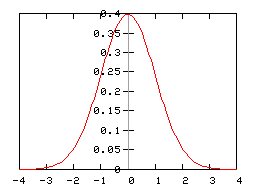
\includegraphics[width=4cm]{gaussreduite.png}}}
}

%************************ Pourqoui Beta ? *********************************
\frame{
\frametitle{Loi pour la durée d'une tâche}

Une loi adéquate est la distribution \textbf{Beta}.
\pause

\begin{center}
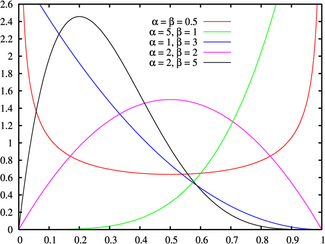
\includegraphics[height=.5\textheight]{betapdf_general.png}
\end{center}

\begin{itemize}
\item<+-> On peut contrôler la forme de la courbe avec $\alpha$ et $\beta$.
\item<+-> En particulier, elle peut être asymétrique (e.g. allongée à droite).
\item<+-> Elle a des limites finies (comme les durées de tâches).
\end{itemize}
}
%************************************************************************
\frame{
\frametitle{Loi pour la durée d'une tâche}

\uncover<1>{Fonction de densité de la distribution:
$$ f(x)=\frac{(x-a)^{p-1}(b-x)^{q-1}}{(b-a)^{p+q-1}B(p,q)} ~~~ a \leq x \leq b ; p,q > 0$$
  	 avec $B$ la fonction beta:
  	 $ B(p,q)=\int_0^1 t^{\alpha-1}(1-t)^{\beta-1} dt$

\vspace{1cm}
}
\pause

Les travaux de C. Clarke (1962) ont donné une méthode pour contrôler
$\alpha$ et $\beta$ à partir de 3 paramètres plus simples : \\
\pause

\begin{tabular}[t]{ll}
	$opt$ : & durée optimiste\\
	$pes$ : &  durée pessimiste\\
	$vrai$ : & durée vraisemblable\\
\end{tabular}

% $$ f(x)=\frac{(x-a)^{p-1}(b-x)^{q-1}}{(b-a)^(p+q-1)B(p,q)} ~~~ 0 \leq x \leq 1 ; p,q > 0$$
%  	 avec $B$ la fonction beta:
%  	 $ B(p,q)=\int_0^1 t^{\alpha-1}(1-t)^{\beta-1} dt$
  	
%
% p = 3 + sqrt{2}    q = 3 - sqrt{2}   si m > (a+b)/2
% p = 3 - sqrt{2}    q = 3 + sqrt{2}   si m > (a+b)/2

}
%************************************************************************
\frame{
\frametitle{PERT probabiliste (2)}
 

Pour une tâche :
\begin{itemize}
\item
Calculer la durée probable d'une tâche $i$ : 
\[
	prob_i = \frac{opt_i + 4~vrai_i + pes_i}{6}
\]
 

\item Mesurer l'incertitude de l'estimation en \\
calculant l'indicateur de dispersion de la durée de la tâche $i$:

\[ d_i = \frac{pes_i - opt_i}{6} \]

\end{itemize}
}
%************************************************************************
\frame{
\frametitle {PERT probabiliste (3)}
Pour un chemin constitué des tâches $\{1;2; ...;n\}$ \\
\begin{itemize}
\item Mesurer la durée estimée du chemin 
\[	D = \sum_{i=1}^n prob_i \]

\item Mesurer l'écart-type de l'estimation pour le chemin :
\[ E = \sqrt{\sum_{i=1}^n d_i^2} \]
\end{itemize}
}
\begin{comment}
Note sur la variance et l'écart-type :
Exemple : on a $k$ notes $\{n_1, ..., n_k\}$. La moyenne est
$m=(\sum_{i=1}^k n_i) /k$.
La variance est $v = (\sum_{i=1}^k (n_i-m)^2)/k$ et l'écart-type
est $\sigma=\sqrt{v}$.
\end{comment}
%************************************************************************
\frame{
\frametitle{PERT probabiliste (4)}

	Obtenir la durée du chemin avec une probabilité $p$ :
	\[ {\cal D}(p) = D + E \times G(p) \] 

où $G$ est la fonction associée à la loi normale centrée réduite (extrait)  :

\[\begin{tabular}{|l|l||l|l|}
\hline
$p$	&	$G(p)$	&$p$		&	$G(p)$ \\
\hline
99,9	& 	3,00    & 89,1		& 	1,23	\\ 
99	& 	2,31	& 85,1		&	1,04	\\
98	& 	2,06	& 70,2		& 	0,53	\\
97	&	1,88	& 50		&	0	\\
95	& 	1,65	& 42,1		& 	-0,2	\\
92,1	&	1,41	& 34,5		& 	-0,4	\\
90	&	1,28	& 27,4		&	-0,6	\\ 		
\hline	
\end{tabular}\]

}
%************************************************************************
\frame{
\frametitle{PERT probabiliste (4)}
\underline{Exemple} : Les estimations sont $D = 100$ et  $E = 15$.\\

	La durée probable à 90\% est
	$$\begin{array}[t]{ll} 
	  {\cal D}(90)	& = 100 + 15 \times G(90) \\
	  		& = 100 + 15 \times 1,28\\
			& \approx 119\\
	\end{array}$$ 


	La durée probable à 70\% est
	$$\begin{array}[t]{ll} 
	  {\cal D}(70)	& = 100 + 15 \times G(70) \\
	  		& = 100 + 15 \times 0,53\\
			& \approx 108\\
	\end{array}$$ 
	
	La probabilité de terminer en 90 jours est
	$$\begin{array}[t]{ll} 
	  90	& = 100 + 15 \times G(p) \\
	  G(p)	& = -10 / 15 = -2 / 3\\
	 \end{array}$$
	d'où ~~~$ p \approx 27\% $ 
}
%************************************************************************
\frame
{\frametitle
{Exercice PERT probabiliste}

\begin{tabular}{|l|l|l|l|l|}
\hline 
$t_i$	& Description	& {\small $opt$}	&  {\small $pes$} & {\small
$vrai$} \\
\hline
$t_1$ & {\small faire fondre le beurre et le chocolat}	& 6	& 9	& 7,5	\\
$t_2$ & {\small séparer les oeufs en jaunes et blancs}	& 1	& 4,5	& 3	\\
$t_3$ & {\small ajouter les jaunes au mélange, faire cuire} & 6 & 8 & 7	\\
$t_4$ & {\small monter les blancs en neige}	& 2 	& 12 	& 5	\\
$t_5$ &	{\small arrêter la cuisson du mélange,}	&	& & \\
      & {\small et incorporer les blancs au mélange}	& 2 & 6 & 3\\
$t_6$ & {\small faire cuire au four}	& 16 & 22 & 18\\
\hline
\end{tabular}

\textit{\small 
\begin{enumerate}
\item Tracer le graphe PERT (sans contrainte de ressources)
\item Calculer la durée probable, l'écart-type de chaque chemin
\item Déterminer le chemin critique
\item Quelle est la durée estimée de préparation du gâteau,
	\begin{itemize}
	\item[--] avec une probabilité de 90\% ?
	\item[--] avec une probabilité de 95\% ?
	\end{itemize}
\item Quelle est la probabilité de terminer en 37 minutes ?	
\end{enumerate}
}
}
%************************************************************************
%* Corrigé
%*
\begin{comment}
      prob   d_i    d_i^2
T1    7.5    1/2    1/4
T2    2.91   0.58   0.34
T3    7      1/3    2/9
T4    5.66   5/3    25/9
T5    3.33   2/3    4/9
T6    18.33  1      1

Examinons les différents chemins :
        +-- T1 --> T3 --+
        |         ^     |
debut --+        /      +--> T5 --> T6 --> fin
        |      /        |
        +-- T2 --> T4 --+
$$
C_1 = \{ T2;T3;T5;T6\}
C_2 = \{ T1;T3;T5;T6\}
C_3 = \{ T2;T4;T5;T6\}

D_{C_1} = 31.57   E_{C_1} = 1.38
D_{C_2} = 36.16   E_{C_2} = 1.34
D_{C_3} = 30.23   E_{C_3} = 2.14

Durée probable avec fiabilité à 90\% , à 95\%
==============================================
{\cal D}(0.9) = D_{C_2} + E_{C_2} * G(0.9)
              = 37.87 (37 min 52 s)
{\cal D}(0.95) = 38,38
=> relativement peu d'incertitude

Comparaison des chemins
=======================
      0.95   0.9
C_1   33.86  33.35
C_2   38.38  37.89
C_3   33.77  32.98

Probabilité x de terminer en 37 min ou moins
============================================
On prend le plus long dans presque (?) tous les cas : C_2
on a :
   {\cal D}(x) = D_{C_2} + G(x).E_{C_2} 
            37 = 36.16 + G(x). 1.34
            G(x) = 0.619
       <=>  x = 72\%

A partir de quelle probabilité x a t-on {\cal D}_{C_3}(x) > {\cal D}_{C_2}(x) ?
==============================================================================
        33.77 + G(x)*2.14    > 36.16 + G(x)* 1.34
        G(x) > 2.98

$$
\end{comment}


%************************************************************************
\subsection{Diagramme Gantt}
\frame{
\frametitle{Diagramme Gantt}
\vspace{.2cm}
\begin{center}
	Etablir un planning
\end{center}
\vspace{.3cm}

\begin{itemize}
\item<+-> Un réseau PERT donne les dates (au plus tôt, au plus tard) sans tenir compte des contraintes de ressources\\
\item<+-> Planning $\Rightarrow$ faire des hypothèses sur les ressources\\
\item<+-> Diagramme Gantt : qui fait quoi et quand ?\\

\item<+-> Possibilité de modifier le planning en 
	\begin{itemize}
	\item jouant sur les ressources affectées
	\item jouant sur le chargement (au plus tôt, au plus tard)
	\end{itemize}
\end{itemize}

}
%************************************************************************
\frame{
\frametitle{Diagramme Gantt (2)}

\input{pert5.pdftex_t}

\underline{Hypothèses} : ressources R1 et R2, et chargement au plus tôt\\
\pause

\input{gantt1.pdftex_t} 

}
%************************************************************************
\frame{
\frametitle {Diagramme de Gantt (3)}

\input{pert5.pdftex_t}

\underline{Hypothèses} : ressources R1 et R2, et chargement au plus tard\\
\pause

\input{gantt2.pdftex_t} 
\vfill
}
%************************************************************************
\frame{
\frametitle{Diagramme Gantt : le nivellement}
\vspace{.4cm}
Le \emph{nivellement} : limiter les ressources utilisées 
 
\vspace{.8cm} 
\begin{center}
\input{gantt4.pdftex_t} 
\end{center}

}
%************************************************************************
\frame{
\frametitle{Diagramme Gantt : le lissage}

\vspace{.3cm}

Le \emph{lissage} : répartir l'utilisation d'une ressource dans le temps

\vspace{.3cm}

\begin{center}
\input{gantt3.pdftex_t} 
\end{center}
}





%
\subsection{Ordonnancement}

\frame{
\frametitle{Ordonnancement}

\begin{itemize}
\item
Affecter des tâches à des ressources dans un ordre,
c'est \textbf{ordonnancer}.

\item
De nombreux résultats proviennent de la recherche opérationnelle.\\
(exemple: Flow job, Job shop.)

\item
Beaucoup des problèmes d'ordonnancement sont NP-complets. \\
Des heuristiques donnant de "bons" résultats souvent utilisées.
\end{itemize}
}


\frame{
\frametitle{Ordonnancement}


Il faut connaître les hypothèses. 
\begin{itemize}
      \item Tâches connues à l'avance ? 
		Si oui, ordonnancement \emph{statique}, si non ordonnancement \emph{online}.
      \item Tâches dépendantes les unes des autres ?
	\item Tâches préemptibles ? préemptible: peut être interrompue.
	\item Ressources hétérogènes ? connaître la capacité de travail de la ressource. 
	\item $\dots$ 
\end{itemize}
}

%---------------------------- Heuristics independent tasks ----------------------------

%----------------------------  Min-min --------------
\subsection{Heuristiques tâches indépendantes}

\frame{
\frametitle{Heuristiques tâches indépendantes}

	Heuristiques tâches indépendantes, Ressources hétérogènes
	\begin{itemize}	
	\item Min-min
	\item Max-min
	\item Sufferage
	\end{itemize}	
}
\frame{
\frametitle{Min-min}
	
\begin{itemize}
\item
	Pour chaque tâche $T_i$, 
     calculer son temps de fin sur toutes les machines et retenir le minimum, appelé $\beta_i$.

\item garder la tâche qui a le temps le plus court: $\stackrel{min}{i}$ $\beta_i$

\item affecter la tâche sur la machine qui donne ce temps

\item recommencer jusqu'à ce que toutes les tâches soient ordonnancées

\end{itemize}	

}



\frame{
\frametitle{Min-min}


%---1--
\only<1,2>{
$$
\begin{array}{|l|l|l|l|}
\hline
		& T_1 & T_2 & T_3  \\
\hline
R_1		& 140	& 20	& 60   \\
\hline
R_2		& 100 & 100 & 70 	\\
\hline
\end{array} $$
}

%---2--
\only<3>{
$$
\begin{array}{|l|l|l|l|}
\hline
		& T_1 &  \textcolor{red}{T_2}  & T_3  \\
\hline
R_1		& {\bf 160}	&  \textcolor{red}{20} &  {\bf 80}   \\
\hline
R_2		& 100 &  --			& 70 \\
\hline
\end{array} $$
}

%---3--
\only<4>{
$$
\begin{array}{|l|l|l|l|}
\hline
		& T_1 &  \textcolor{red}{T_2}  & \textcolor{blue}{T_3}  \\
\hline
R_1		& 160	&  \textcolor{red}{20} &  --   \\
\hline
R_2		& 100 &  --				& \textcolor{blue}{70} \\
\hline
\end{array} $$
}
%---3--
\only<5>{
$$
\begin{array}{|l|l|l|l|}
\hline
		& T_1 &  \textcolor{red}{T_2}  & \textcolor{blue}{T_3}  \\
\hline
R_1		& 160	&  \textcolor{red}{20} &  --   \\
\hline
R_2		& {\bf 170} &  --				& \textcolor{blue}{70} \\
\hline
\end{array} $$
}

%---7--
\only<6>{
$$
\begin{array}{|l|l|l|l|}
\hline
		& \textcolor{brown}{T_1} &  \textcolor{red}{T_2}  & \textcolor{blue}{T_3}  \\
\hline
R_1		& \textcolor{brown}{160}	&  \textcolor{red}{20} &  --   \\
\hline
R_2		& 170 &  --				& \textcolor{blue}{70} \\
\hline
\end{array} $$
}

\pause
\begin{itemize}
\item<+-> $T_2$ sur $R_1$ (20)
\item<+-> tâches sur $R_1$ vont terminer 20 unités de temps plus tard
\item<+-> $T_3$ sur $R_2$ (70)
\item<+-> tâches sur $R_2$ vont terminer 70 unités de temps plus tard
\item<+-> $T_1$ sur $R_1$ (160)
\end{itemize}
}


%----------------------------  Max-min --------------

\frame{
\frametitle{Max-min}

Soit $T$ l'ensemble des tâches à ordonnancer.
\begin{itemize}
\item
Pour chaque tâche $T_i \in T$ 
     calculer son temps de fin sur toutes les machines et retenir le minimum, appelé $\beta_i$.

\item garder la tâche qui a le temps de fin maximum: $\underset{i}{max}$ $\beta_i$

\item affecter la tâche sur la machine qui donne ce temps

\item recommencer avec l'ensemble $T \backslash T_i$,
       jusqu'à ce que toutes les tâches soient ordonnancées

\end{itemize}	

}



\frame{
\frametitle{Exemple Max-min}

%---1--
\only<1,2>{
$$
\begin{array}{|l|l|l|l|}
\hline
		& T_1 & T_2 & T_3  \\
\hline
R_1		& 140	& 20	& 60   \\
\hline
R_2		& 100 & 100 & 70 	\\
\hline
\end{array} $$
}

%---2--
\only<3>{
$$
\begin{array}{|l|l|l|l|}
\hline
		& \textcolor{red}{T_1} &  T_2  & T_3  \\
\hline
R_1		& --	&  		20 &   60 \\
\hline
R_2		& \textcolor{red}{100} &  200	& 170 \\
\hline
\end{array} $$
}

%---3--
\only<4>{
$$
\begin{array}{|l|l|l|l|}
\hline
		& \textcolor{red}{T_1} &  T_2  & \textcolor{blue}{T_3}  \\
\hline
R_1		& --	&  		20 &   \textcolor{blue}{60} \\
\hline
R_2		& \textcolor{red}{100} &  200	& 170 \\
\hline

\end{array} $$
}


%---3--
\only<5>{
$$
\begin{array}{|l|l|l|l|}
\hline
		& \textcolor{red}{T_1} &  T_2  & \textcolor{blue}{T_3}  \\
\hline
R_1		& --	&  		{\bf 80}  &   \textcolor{blue}{60} \\
\hline
R_2		& \textcolor{red}{100} &  200	& 170 \\
\hline
\end{array} $$
}

%---7--
\only<6>{
$$
\begin{array}{|l|l|l|l|}
\hline
		& \textcolor{red}{T_1} &  \textcolor{brown}{T_2}  & \textcolor{blue}{T_3}  \\
\hline
R_1		& --	&  \textcolor{brown}{80}	  &   \textcolor{blue}{60} \\
\hline
R_2		& \textcolor{red}{100} &  200	& 170 \\
\hline
\end{array} $$
}

\pause
\begin{itemize}
\item<+-> $T_1$ sur $R_2$ (100)
\item<+-> tâches sur $R_2$ vont terminer 100 unités de temps plus tard
\item<+-> $T_3$ sur $R_1$ (60)
\item<+-> tâches sur $R_1$ vont terminer 60 unités de temps plus tard
\item<+-> $T_2$ sur $R_1$ (80)
\end{itemize}
}


\begin{comment}
\subsection{Heuristiques tâches dépendantes}

\frame{
\frametitle{}
	Heuristiques tâches dépendantes, Ressources hétérogènes
	\begin{itemize}	
	\item HEFT 
	\item 
	\item 
	\end{itemize}	
}

\end{comment}


		
	
\end{document}  
